\section{偏序格}
设\(\opair{L,\leq}\)是偏序集,\(\leq\)是\(L\)上的偏序关系,
\(L\)中的两个元素的上确界及下确界不一定存在.
例如,由哈斯图 \labelcref{figure:格论.偏序集1} 可知,
\(\{c,b\}\)无上确界,\(\{a,d\}\)无下确界.

\begin{figure}[htb]
%@see: 《离散数学》(邓辉文) P155 图5-1
	\centering
	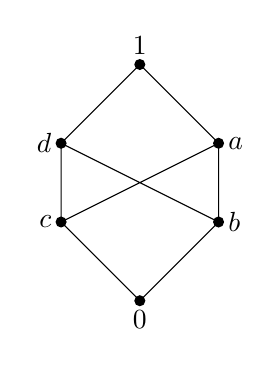
\begin{tikzpicture}
		\fill(0,0)circle(2pt);
		\fill(1,-1)circle(2pt);
		\fill(1,-2)circle(2pt);
		\fill(-1,-1)circle(2pt);
		\fill(-1,-2)circle(2pt);
		\fill(0,-3)circle(2pt);
		\draw(0,0)node[above]{$1$}
			--(1,-1)node[right]{$a$}
			--(1,-2)node[right]{$b$}
			--(0,-3)node[below]{$0$}
			--(-1,-2)node[left]{$c$}
			--(-1,-1)node[left]{$d$}--(0,0)
			(-1,-1)--(1,-2) (1,-1)--(-1,-2);
	\end{tikzpicture}
	\caption{}
	\label{figure:格论.偏序集1}
\end{figure}

\begin{definition}
%@see: 《离散数学》(邓辉文) P155 定义5-19
设\(\opair{L,\leq}\)是偏序集.
若\(L\)中任意两个元素都存在上确界和下确界,
则称\(\opair{L,\leq}\)是\DefineConcept{偏序格}(lattice).
%TODO 缺少定义:偏序集中任意两个元素的上确界、下确界
%@see: https://mathworld.wolfram.com/Lattice.html
\end{definition}

\begin{example}
%@see: 《离散数学》(邓辉文) P155 例5-27
设\(X\)是非空集合.
证明:\(\opair{\Powerset X,\subseteq}\)是偏序格.
\begin{proof}
显然\(\opair{\Powerset X,\subseteq}\)是偏序集.
对于任意\(A,B \in \Powerset X\),有\[
	\sup\{A,B\}
	= A \cup B
	\in \Powerset X,
	\qquad
	\inf\{A,B\}
	= A \cap B
	\in \Powerset X,
\]
所以\(\opair{\Powerset X,\subseteq}\)是偏序格.
\end{proof}
\end{example}
